\chapter{Introduction}
\labch{intro}
	\section{Purpose}
		During their university studies, in order to start entering the workforce, a student might decide to apply for an internship related to their field of study. Similarly, companies offering internships may be interested in finding students that are adequate for them. To facilitate the matching between students and companies, a new platform called \emph{Students and Companies} (S\&C) is to be developed. S\&C allows companies to look for suitable students by publish internship advice on the platform, while students can look for internships that interest them. Moreover, the platform implements recommendation mechanism to help student and companies to find each other. Once the contact is established, S\&C can provide support to the students selection process and in monitoring the status of outgoing internships.
		\subsection{Goals}
			The main goals of the system are:
			
			\quad [G1]\quad students and companies establish contacts for doing internships;
			
			\quad [G2]\quad internships selections can be monitored and supported by the system;
			
			\quad [G3]\quad ongoing internships can be monitored from the system.
	\section{Scope}
		In this section, we are identifying the S\&C domain. In particular, there are two main users categories that interact with the system: \emph{Companies} and \emph{Students}. The companies publish announcements about the internships they want to offer where they specify \emph{projects} that will be carried out and the \emph{terms} of the offer. The system itself informs the companies about the availability of students who may be suitable for their internships (based on their profile).
		
		Students, on the other hand, may use the platform to look for internships and S\&C can also notify them if there are new internships that could meet their interests, but they can still independently search through all the available internships.
		
		Once a \emph{contact} is established and accepted by the two parties, the student selection process begins. At this point the company defines selection steps and schedules the interviews for each student. Once the selection is over, the system collects feedback and suggestions from both students and companies.
		
		Finally, both students and companies can monitor the progress of the internships by providing information on its development and any issues that may arise. At the end of the internship, both students and companies can provide feedback about the internship; this feedback are collected by the system and, through some statistical analysis on them, used to improve the recommendation mechanism.
		\subsection{Phenomena}
			\subsubsection{World Phenomena}
				[WP1] Students create their own CV, including their studies, work experiences, skills, and attitudes
				
				[WP2] Company decides to offer a new internship for students who want to gain experience
				
				[WP3] During the selection process, the company conducts an interview with the student
				
				[WP4] Students selected for a particular internship begin working on the related projects
				
				[WP5] Users of the platform (students and companies) encounter issues with the internship projects they are working on
			\subsubsection{Shared Phenomena}
				\paragraph{World-controlled Shared Phenomena}
					\begin{flushleft}
											[SP0] Users register to the platform by providing email, password and all the information necessary to their profile creation (e.g. CV for students, business area for companies ecc.)
											
											[SP1] Companies publish new internship advice
											
											[SP2] Students search for all the available internships on the platform
											
											[SP3] Students search for all the companies registered on the platform
											
											[SP4] Students search for specific internships using the search bar
											
											[SP5] Students apply for an internship
											
											[SP6] Companies accept/decline the applications of some students for their internships
											
											[SP7] Companies offer internship proposals to specific students
											
											[SP8] Students accept/decline the internship application offer
											
											[SP9] Companies configure the selection process for their internships
											
											[SP10] Companies enter the evaluations of the students' interview answers
											
											[SP11] Students are selected/rejected by the selection process's company 
											
											[SP12] Users (students and companies) provide feedback and suggestions about the internship and the selection processes
											
											[SP13] Users (students and companies) monitor the status of ongoing internships, providing complaints, problems and information about them
											
											[SP14] Companies delete their internship advice
											
											[SP15] Companies close their concluded internships
 					\end{flushleft}
				
				

					
					
				\paragraph{Machine-controlled Shared Phenomena}
					\begin{flushleft}
						[SP16] The system notifies companies when a student applies for one of their advice
						
						[SP17] The system notifies students when an internship that might interest them become available
						
						[SP18] The system notifies companies about the availability of interesting students regarding their internships
						
						[SP19] The system notifies students if the companies accept their application for the internships
						
						[SP20] The system notifies companies if the students accept their application proposal for the internships
					
						[SP21] The system notifies students about the interview dates
						
						[SP22] The system notifies students their selection final result
						
						[SP23] The system notifies users when an ongoing internship the interest them is concluded
						
						[SP24] The system calculates and shows to companies selections steps results
						
						[SP25] The system perform recommendation analysis
					\end{flushleft} 
					
					%[SP20] The system collects the complaints provided by the users (students and companies) about ongoing internships
	\section{Definitions, Acronyms and Abbreviations}
		\subsection{Definitions}
			\begin{itemize}
				\item \textbf{internship advice} : a call for application related to an internship that will be offered by a company;
				\item \textbf{recommendation} : the mechanism related to the fact that the system both informs students whether new internship advice that might interest them are published and notifies companies of the presence of students that might be suitable for their internships;
				\item \textbf{contact}: a student and a company establish a contact when the company accepts the application of the student or the student accepts the proposal of application of the company
				\item \textbf{project} (of an internship advice) : the definition of the application domain, the set of tasks to be performed and the set of the most relevant adopted technologies (if any) for an internship;
				\item \textbf{terms} (of an internship advice) : the set of benefits offered by an internship (e.g. paid/not paid, training, lunch voucher... );
				\item \textbf{selection process} : each internship advice is followed by a sequence of selection steps;
				\item \textbf{platform}: synonym of \text{system};
				\item \textbf{notification} : it is a message sent to an user that the user can consult on its private area. Note that with the term \emph{notification} we don't refer to the e-mail sent to the user, but only to the message it can consult once logged into the platform.
			\end{itemize}
		\subsection{Acronyms}
			\begin{itemize}
				\item S\&C: Students\&Companies, the name of the platform;
				\item UML: Unified Modeling Language;
				\item CV: Curriculum Vitae.
			\end{itemize}
		\subsection{Abbreviations}
			\begin{itemize}
				\item Gn: Goal number n;
				\item Rn: Requirement number n;
				\item Dn: Domain assumption number n;
				\item WPn: World Phenomena number n;
				\item SPn: Shared Phenomena number n;
				\item UC: Use Case.
			\end{itemize}
	\section{Revision history}
		\begin{center}
			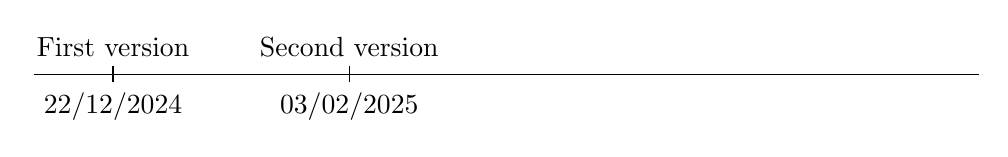
\begin{tikzpicture}
				% draw a horizontal line
				\draw (0,0) -- (12,0);
				
				% draw vertical lines
				\foreach \x in {1,4}
				\draw (\x cm,3pt) -- (\x cm,-3pt);
				
				% draw nodes to add events
				\draw (1,0) node[below=3pt] {22/12/2024} node[above=3pt] {First version};
				\draw (4,0) node[below=3pt] {03/02/2025} node[above=3pt] {Second version};
			\end{tikzpicture}
		\end{center}
		
		In version 2 we uniformed the application sections names, in order to prevent possible ambiguities.
	\section{Reference documents}
		The Documents used to deliver the RASD document are the following:
		\begin{itemize}
			\item the Specification of RASD and DD assignment of Software Engineering 2;
			\item the class slides on WeBeep, in particular slides on RE (requirement engineering), scenarios and Use Cases and UML diagrams;
		\end{itemize}
	\section{Document structure}
		\begin{enumerate}
			\item \textbf{Introduction}: this section provides a brief introduction to the purpose of the platform to be developed, S\&C in this case, focusing in particular on the most important goals which the system has to achieve and on the various phenomena identified;
			\item \textbf{Overall Description} : an high-level (conceptual) description of the system functionalities explained through scenarios, high-level class diagram, product functions and domain assumption;
			\item \textbf{Specified Requirements} : the detailed requirements analysis. In this section is detailed the entire requirement set (functional and non-functional), the most relevant use-cases (including sequence diagrams that formalize them) and the design constraints that must be stated also at the requirement level;
			\item \textbf{Formal Analysis} : formal modeling and simulation of a simplified model of the system, in order to formally prove the correctness of the (possibly) foremost requirements (using Alloy 6);
			\item \textbf{Effort Spent}: report of the time spent by any group member in any document section;
			\item \textbf{Software Used}: list of software used to develop the document.
		\end{enumerate}